%\documentclass[]{spie}  %>>> use for US letter paper
\documentclass[a4paper,nocompress]{spie}  %>>> use this instead for A4 paper
%\documentclass[nocompress]{spie}  %>>> to avoid compression of citations

\renewcommand{\baselinestretch}{1.0} % Change to 1.65 for double spacing
 
\usepackage{amsmath,amsfonts,amssymb}
\usepackage{graphicx}
\usepackage[colorlinks=true, allcolors=blue]{hyperref}
\usepackage[dvipsnames]{xcolor}
\usepackage{tabularx}
\setlength{\extrarowheight}{2pt}
\usepackage{chemformula}

\title{Quantifying the Impact \\ of Performance Improvements and Cost Reductions \\ from 20 years of Light-Emitting Diode Manufacturing}

\author[a,b]{Michael Weinold}
\author[b]{Sergey Kolesnikov}
\author[b,c]{Laura Diaz Anadon}
\affil[a]{Chair of Entrepreneurial Risks, ETH Zurich, Scheuchzerstrasse 7, CH-8092 Zurich, CH}
\affil[b]{Centre for Environment, Energy and Natural Resource Governance, Department of Land Economy, University of Cambridge, Cambridge, CB3 9EP, UK}
\affil[c]{Belfer Center for Science and International Affairs, Harvard Kennedy School, Harvard University, Cambridge, MA 02138, USA}

\authorinfo{Further author information: (Send correspondence to Michael Weinold) \\ MW: E-mail: mw799@cam.ac.uk \\ SK: E-mail: sk2063@cam.ac.uk \\ LDA: E-mail: lda24@cam.ac.uk}

% Option to view page numbers
\pagestyle{empty} % change to \pagestyle{plain} for page numbers   
\setcounter{page}{301} % Set start page numbering at e.g. 301
 
\begin{document} 
\maketitle

\begin{abstract}
    
    With the aim of identifying and quantifying the principal sources of performance improvements and cost reductions in white light emitting diode manufacturing, we collect historical data on device cost and performance, technological breakthroughs and manufacturing innovation for phosphor-converted white light-emitting diodes for the past 20 years. We find that technological breakthroughs and process innovation contributed to performance improvements across the entire range of LED device sub-efficiencies, resulting in the overall increase in the lamp efficiency for the highest performing devices at a test current of 350mA from 5.8\% to 38.7\% between 2002 and 2020. We further develop a bottom-up manufacturing cost model with process-step resolution that captured improvements in throughput, yield and related costs of all relevant manufacturing steps, as well as economies of scale, to analyse progress in LED manufacturing cost structure between early manufacturing in 2003 and 2020. We estimate that the cost of manufacturing low-power and mid-power light-emitting diode packages at a US location using state-of-the-art equipment has dropped from 1.11\$(2020) in 2002 to 0.05\$(2020) in 2020, a 95.5\% decrease. We also find that the largest contribution to overall cost reductions has come from increase in wafer size, and that in 2020, chip packaging remains the largest contributor to cost at 60\%.

\end{abstract}

% Include a list of keywords after the abstract 
\keywords{light-emitting diodes, LED manufacturing, LED efficiency, manufacturing cost, cost modeling, cost reduction, technological breakthroughs}

\section{INTRODUCTION}
\label{sec:intro}


    Within only 25 years of the introduction of the first commercial white light-emitting diode, efficiency has increased by three orders of magnitude while manufacturing costs have fallen by two orders of magnitude. After legislation aimed at increasing the adoption of solid-state light sources has been implemented around the world, the solid state lighting industry has become a rare success story in the global drive for the transformation of energy systems. Estimates for the electrical energy saved annually from the adoption of energy efficiency lamps ranges from 131 TWh/year in 2020 for the EU \cite{eu2019impactass} to 442 TWh/year in 2020 for the US \cite{yamada2015adoption,guidehouse2020adoption}. 
    
    Understanding the sources and impact of these dramatic improvements on LED manufacturing is essential for researchers, industry professionals, as well as policymakers in the sphere of energy, science and innovation, as they may provide valuable insights for the acceleration of innovation in other demand-side energy technologies. Our research aims to XXX


\clearpage
\section{Methods and Data}
\label{sec:methods}

\subsection{Choice of Metrics}

    To describe the effect of technological breakthroughs and manufacturing process improvements, a set of metrics had to be identified. The ensemble of metrics is required to describe all dimensions of device performance, including the overall physical device efficiency and the sub-efficiencies related to different physical loss channels. They must further have the ability to directly describe the effect of single technological breakthroughs, evolution in device architecture and manufacturing process improvements on device performance.
    
    These requirements precluded the use of some established metrics. For instance, a highly cited and frequently updated metric is the total luminous flux per light-emitting diode package \cite{Liu2009,haitz2011solid,cho2017white,Fontoynont2018}. In combination with the cost per total flux, it is sometimes referred to as \textit{"Haitz's Law"}, in reference to an early report on LED development by Haitz et al. \cite{haitz1999case}. However, while it is often used to showcase technological progress in light-emitting diode design and manufacturing, care must be taken to consider its limitations.
    
    Firstly, the metric today retains only limited significance as a proxy for technological development in light-emitting diodes. This is because it is not desirable to increase the total flux per device beyond a certain point in many applications. Reasons for limiting the total flux per device may include lighting design considerations to reduce glare \cite{khan2015led}, device efficiency considerations to avoid electrical droop at high operating currents associated with high brightness \cite{Piprek2010} and economical considerations where multiple LED die in a single package can achieve the same brightness as a single high-brightness LED die. Secondly, disregarding these limitations, the total flux per device would only be a proxy for technological improvements in light-emitting diodes, if data was given for single light-emitting diode chips, instead of multi-chip packages. Historically, publications have sometimes failed to make this distinction, listing datapoints for both device levels in the same graph without supporting information.

    Figure \ref{fig:haitz} shows an updated and expanded overview of the flux per device and the cost per flux of highest performing light-emitting diodes, both at the chip and package level, to demonstrate the limitations of these metrics. It is evident that the historical improvement in total flux per package for single chips is not as pronounced as for multi-chip packages.

    \begin{figure} [ht]
        \begin{center}
            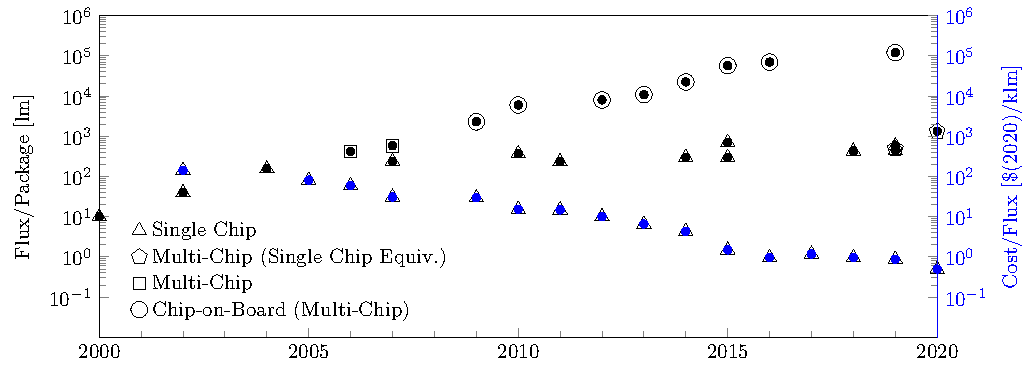
\includegraphics[width=\textwidth]{haitz_law_white.pdf}
        \end{center}
        \caption{Historical increase in flux for highest performing white light-emitting diode chips and (multi-chip) packages, inspired by \textit{"Haitz's Law"}\cite{haitz1999case}. Shown are datapoints for best commercial performers from press releases, datasheets and and industry periodicals. Note the logarithmic ordinates and the black colored datapoints corresponding to the left ordinate, blue colored datapoints corresponding to the right ordinate.}
        \label{fig:haitz}
    \end{figure}

    \clearpage
    Instead, progress in light-emitting diode technology is best described by the overall device efficiency, or lamp efficiency. This metric is defined as the product of all device sub-efficiencies associated with an ensemble of different loss channels $\eta_L = \prod_{i=(V_f,\dots,S)} \eta_i$. Sub-efficiencies directly capture the effect of particular technological breakthroughs in device design and manufacturing process improvements. Table \ref{tab:eff} lists the relevant sub-efficiencies considered along with mathematical definitions.
    
        \begin{table}[h!]
        \caption{List of the device sub-efficiencies used in our methodology. We follow the definitions used by previous authors, such as Tsao et al. \cite{tsao2010solid} and Pattison et al. \cite{pattison2017solid}. The historical development of the sub-efficiencies is displayed in figure \ref{fig:efficiency}.}
        \bigskip
        \centering
    	\begin{tabularx}{\textwidth}{|l|l|l|X|}
    		\hline
    			\textit{Symbol} & \textit{Sub-Efficiency} & \textit{Loss-Channel} & \textit{Definition} \\
    		\hline
    		    $\eta_{V_f}$ & Forward Voltage Efficiency* & Ohmic Resistance & $\eta_{V_f} = E_{h\nu} / V_f $ \\
    		\hline
    		    $\eta_{LE}$ & Light-Extraction Efficiency & Re-absorption and Reflection & $\eta_{LE}= P_{out} / P_{in} $ \\
    		\hline
    		    $\eta_{IQ}$ & Internal Quantum Efficiency & Non-radiative Recombinations & $\eta_{EQ} = \eta_{IQ} \times \eta_{LE}$ \\
    		\hline
    		    $\eta_{Droop}$ & (Electrical) Droop & Non-radiative Recombinations & $\eta_{Droop} = 1 - \eta_{IQE} / \eta_{IQE}(A \rightarrow 0) $ \\
    		\hline
    		    $\eta_C$ & Conversion Efficiency & Stokes Loss, Absorption, etc. & $\eta_{C} = E_{\textcolor{blue}{B}} / \sum_{i=\textcolor{red}{R},\textcolor{orange}{O},\textcolor{yellow}{Y},\textcolor{teal}{G}} E_i$ \\
    		\hline
    		    $\eta_{S}$ & Spectral Efficiency & Eye Sensitivity & $\eta_{S} = K / K_{max}(CRI,CCT)$ \\
    		\hline
    		    $\eta_L$ & Lamp Efficiency & N/A (Cumulative) & $\eta_L = \prod_{i=(V_f,\dots,S)} \eta_i$ \\
            \hline
                \multicolumn{4}{|l|}{$\!\begin{aligned}
                    E_{h\nu} &\dots \text{photon energy} \\
                    V_f &\dots \text{forward voltage} \\
                    A &\dots \text{electrical current} \\
                    E_{B,\dots,G} &\dots \text{optical energy of monochromatic light (blue, red, orange, yellow, green)} \\
                    K &\dots \text{luminous efficacy of radiation} \\
                    CRI &\dots \text{color rendering index}, \ CCT \dots \text{color temperature} \\
                \end{aligned}$} \\
            \hline
    	\end{tabularx}
    	\label{tab:eff}
    \end{table}
    
    Performance improvements in metrics related to consumer experience have also played a role in the adoption of light-emitting diode based luminaires \cite{cowan2011understanding}. Broadly described as the quality of light, these include metrics related to the emitted spectrum as well flicker, the temporal modulation of light. For instance, breakthroughs in the development of downconversion phosphors enabled a greater range in the color temperature of light sources. The work on analyzing consumer experience metrics is ongoing and will be presented in our future work. Notably, we exclude flicker from this context because it is not an inherent property of the light-emitting diodes themselves, but rather the electrical ballasts in the luminaires. We instead refer to a recent publication by Weinold \cite{weinold2020long}.

    \subsection{Data Sources and Performance Calculations}
    \label{subsec:data}
    
        To gain a detailed understanding of the sources and magnitude of efficiency improvements and cost reductions in light-emitting diode manufacturing, we gathered data from a variety of sources. The aim was to collect historical data on overall device performance and historical development in sub-efficiencies. Where possible, we gathered  efficiency data from literature or computed the respective values from raw data. We further had to identify the associated device architectures, manufacturing processes and types of down conversion phosphors used. Data was extracted from patent literature, scientific publications, industry reports and technology forecasts. Additional information and data was provided by experts from both the light-emitting diode manufacturing industry and the manufacturing equipment industry during semi-structured interviews. 
        
        For instance, to gather historical data on the reduction of losses associated with electrical droop, device performance data was calculated based on the information extracted from datasheets, as shown in figure \ref{fig:droop}. This data was cross-referenced with information on the different chip architectures and manufacturing processes used for each device. This data was then augmented by data provided in industry reports and company publications \cite{osram2014osram}. Data was gathered in a similar way for all sub-efficiencies listed in table \ref{tab:eff}, to gather a complete picture of the historical development of light-emitting diode efficiency.

        \begin{figure} [ht]
            \begin{center}
                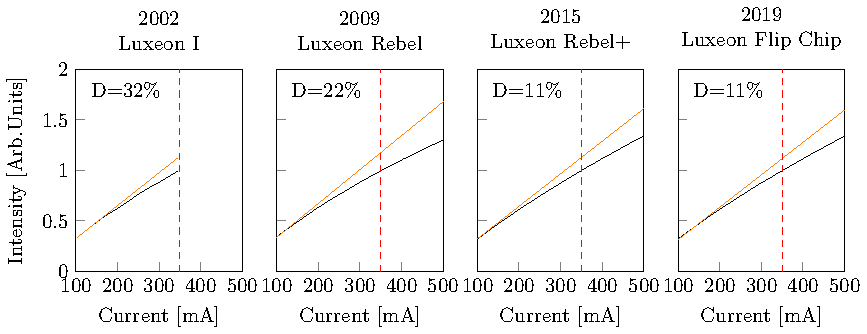
\includegraphics[width=0.85\textwidth]{SPIE/article/droop_lumileds.pdf}
            \end{center}
            \caption{Luminous intensity of four different \textit{Lumileds} high-power light-emitting diodes normalized to the value at a test current of $A_{test}=350$mA. The black curves describe the real measured intensity, the orange curves describe the estimated ideal intensity. Droop $D$, as defined in table \ref{tab:eff}, is the difference between these curves at the test current. Current-Intensity data extracted from device datasheets \cite{datasheet_lumileds_lux1,datasheet_lumileds_rebel,datasheet_lumileds_rebplus,lumi2019data}}
            \label{fig:droop}
        \end{figure}



    \subsection{Manufacturing Cost Model}

        To quantify changes in the manufacturing cost of devices, a bottom-up manufacturing cost model with process step resolution was constructed. It covers the entire manufacturing process of GaN-on-sapphire-based phosphor-converted low-to-mid power light-emitting diode packages of different chip architectures. We considered the classical p-side-up lateral current spreading architecture, as well as a packaged flip-chip vertical current spreading architecture and a chip-scale package flip chip architecture. An excerpt of the device architectures considered is shown in figure \ref{fig:chip_arch}. The earliest commercial warm-white phosphor converted blue light emitting diodes were introduced in 2003, so the model was constructed for the years 2003, 2012 and 2020. It was populated with equipment data from European and North American firms, selected for a virtual North American manufacturing location. Details of the manufacturing processes and process-specific step parameters were derived from the sources mentiond in section \ref{subsec:data}. For 2012, additional data for the model was adapted from the \textit{LEDCOM} cost model prepared for the US Department of Energy by Stephen Bland of SB Consulting\cite{ledcomv2}. Our model includes both the wafer treatment process as well as the packaging process. While the model offers great flexibility to researchers in adapting the manufacturing process parameters and chip architectures used, it is important to note the limitations of this approach. The main aim of the model is not to faithfully represent real-world manufacturing such as those in present-day manufacturing locations in Asia, but rather to show the effect of technological change and manufacturing process improvements on total cost. 

        \begin{figure} [ht]
            \begin{center}
                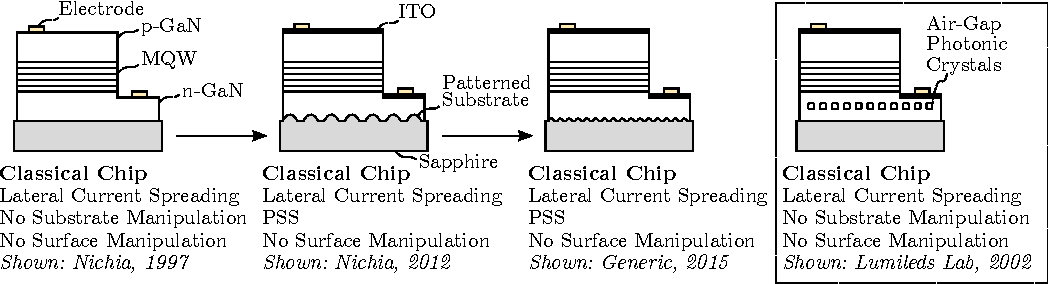
\includegraphics[width=\textwidth]{SPIE/article/chip_architectures.pdf}
            \end{center}
            \caption{Cutaway side views of the evolution of chip architectures for classical chip designs (lateral current spreading). Note that dimensions are not to scale. Years correspond to earliest identified patent priority date. Dashed boxes indicate chip designs not brought to large scale production. Adapted from patents \cite{nagahama2013nitride,tanaka2010semiconductor,wierer2006photonic}}
            \label{fig:chip_arch}
        \end{figure}

        To dis-aggregate the contribution of changes in single variables to changes in the total manufacturing cost, we used an approach introduced by Kavlak et al. in a cost model for photovoltaic modules \cite{kavlak2018evaluating}. It is based on the logarithmic derivative of the total differential of the cost function.  For the detailed derivation, we refer to the supplementary material of the original publication.

\section{RESULTS}

\subsection{Performance Improvements}

     Results for performance improvements are presented in Figure \ref{fig:efficiency}. Overall efficiency in best performing devices improved from $\eta_L=5.8\%$ in 2002 to $\eta_L = 38.7\%$ in 2020. As previous studies have noted, no single loss channel dominates the overall the efficiency\cite{tsao2010solid}. Figure \ref{fig:efficiency} additionally shows the physical limits for the loss channels. We note, that those loss channels with a fixed physical limit below 100\% have become significantly more dominant in 2016 and 2020. For instance, Stokes loss, describing the energy dissipated upon conversion from short wavelength to long wavelength photons, becomes more dominant. Notably, sub-efficiencies for the most current devices are only $\sim10\%$ below the physical limit. The exception is spectral efficiency, which at $\sim20\%$ below the physical limit shows larger potential for improvement.
     
     Our comparison between the improvements in device sub-efficiencies between 2002 and 2020 shows that the aggregate efficiency improvement was not driven primarily by improvements in a single sub-efficiency. Instead, there has been consistent progress across the ensemble of loss channels corresponding to the device sub-efficiencies in the past 18 years: forward voltage efficiency ($70\%\rightarrow99.5\%$), internal quantum efficiency ($55\%\rightarrow90\%)$, electrical droop ($65\%\rightarrow90\%$), light-extraction efficiency ($60\%\rightarrow90\%$) and spectral efficiency ($74\% \rightarrow83\%$).
     
     XXX video text
     
    \begin{figure} [ht]
        \begin{center}
            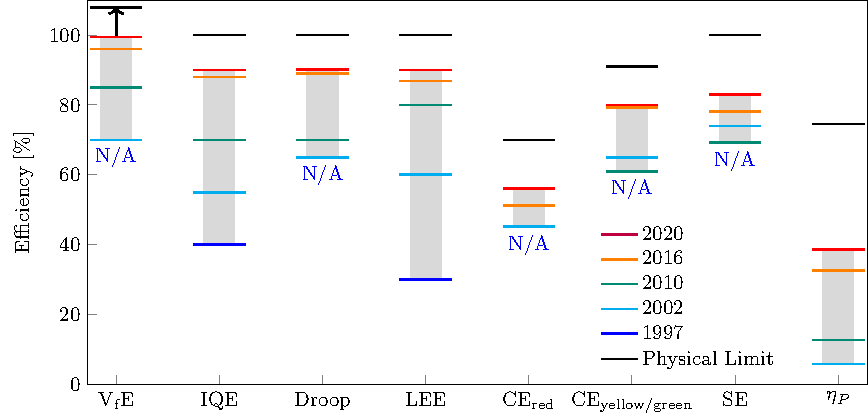
\includegraphics[width=0.85\textwidth]{SPIE/article/breakthroughs_efficiency.pdf}
        \end{center}
        \caption{Impact of technology breakthroughs and manufacturing process improvements on historical developments in sub-efficiencies of phosphor-converted warm white light-emitting diodes with test currents of at least $I_\text{test}=350$mA. The overall lamp efficiency $\eta_L$ is displayed as the rightmost column. This figure takes as inputs the state-of-the-art sub-efficiencies discussed in section \ref{sec:methods}. Horizontal colored bars give state-of-the-art sub-efficiencies for five years: \textcolor{blue}{1997}, \textcolor{teal}{2002}, \textcolor{orange}{2010}, \textcolor{magenta}{2016} and \textcolor{red}{2020}. Colored annotation "N/A" indicates that the sub-efficiency of the corresponding year cannot be computed for the following reasons: V$_\text{f}$E, Droop: depend on current, which was below 350mA at the time; CE, SE: warm white spectrum LEDs not available at the time. Physical limits are indicated by black horizontal bars. The possible range for the physical limit of V$_\text{f}$E exceeds 100\% and depends on electrical device parameters, which are discussed in \cite{david2016electrical}. The range of this limit is indicated by an upward pointing black arrow. Efficiency acronyms are listed in table \ref{tab:eff}. Data for historical improvements of sub efficiencies from Weinold et al. \cite{weinold2020technology}}
        \label{fig:efficiency}
    \end{figure}

\subsection{Manufacturing Cost Reductions}

    Using our cost model, we estimate that the cost of manufacturing low-power and mid-power light-emitting diode packages at a US location, using state-of-the-art equipment, to have decreased from 1.11\$(2020) in 2002 to 0.05\$(2020) in 2020, a 95.5\% decrease. 
    
    A preliminary analysis of components of the cost model suggests that an increase in wafer size in the manufacturing process is responsible for the largest part of the cost reduction. The number of die per wafer associated with this is displayed in the inset plot of figure \ref{fig:cost}. The wafer diameter used in production has been steadily increasing since 2002. The model assumes diameters and associated number of die per wafer  $d(2002)=50$mm$\rightarrow851$ to $d(2020)=200$mm$\rightarrow26,838$. Note that the decrease in exclusion zone and cutting width also contribute to the increase in die per wafer.
    
    As the number of die per wafer increases, the packaging steps carry a larger share of the total cost. This is because these steps are limited by the throughput of the associated equipment. The wafer processing steps are limited by the number of die per wafer and only to a lesser extend the throughput of equipment.

\begin{figure} [ht]
    \begin{center}
        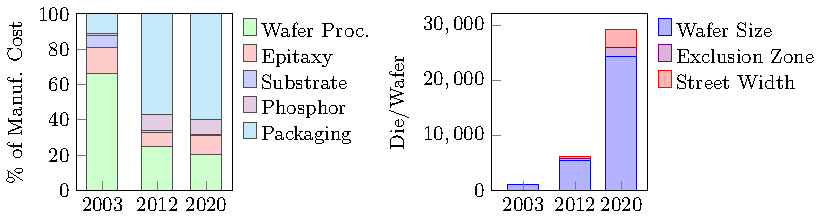
\includegraphics[width=0.85\textwidth]{SPIE/article/costmodel_calibration.pdf}
    \end{center}
    \caption{Modeled manufacturing cost for the specified architecture of light-emitting diode packages split by manufacturing step category, following the categories and color scheme used in the reports by the US DoE \cite{doe2016solid}. The inset plot shows the number of die per wafer corresponding to wafers of different sizes, associated street width and exclusion zone. Calculated using approximations introduced by de Vries \cite{deVries2005}.}
    \label{fig:cost}
\end{figure}

    \subsection{Future Work}


\acknowledgments % equivalent to \section*{ACKNOWLEDGMENTS}       

We express our gratitude to all inteviewees for their willingness to participate in this study and invaluable contributions. This research is funded by the \textit{Alfred P. Sloan Foundation} of New York, USA, grant number 253128. Michael Weinold further gratefully acknowledges support from the \textit{Swiss Study Foundation} of Zurich, Switzerland.


\clearpage
% References
\bibliography{report} % bibliography data in report.bib
\bibliographystyle{spiebib} % makes bibtex use spiebib.bst

\end{document} 
